\paragraph{QuizziPedia::Back-End::App::Models::QuestionModel}
\label{QuizziPedia::Back-End::App::Models::QuestionModel}
\begin{figure}[ht]
	\centering
	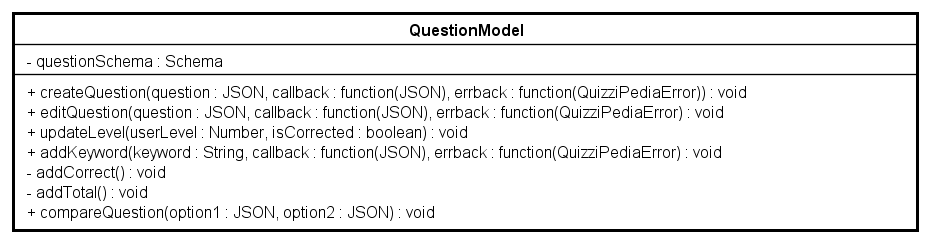
\includegraphics[scale=0.45]{UML/Classi/Back-End/QuizziPedia_Back-End_App_Models_questionModel.png}
	\caption{QuizziPedia::Back-End::App::Models::QuestionModel}
\end{figure}
\FloatBarrier
	\begin{itemize}
		\item \textbf{Descrizione} \\
		Classe che modella i dati relativi alle domande all'interno dell'applicazione;	
		\item \textbf{Utilizzo} \\
		Viene utilizzata per rappresentare le domande. Si interfaccia alla libreria \textit{Mongoose\ped{G}} per la creazione dello schema e dei relativi metodi statici o di istanza;
		\item \textbf{Relazione con altra classi}:
			\begin{itemize}
			\item IN \textbf{UserModel} \\
			Classe che rappresenta tutti gli utenti;
			\item OUT \textbf{SummaryModel} \\
			Classe che rappresenta i riepiloghi dei questionari svolti;
			\item OUT \textbf{TopicModel} \\
			Classe che rappresenta gli argomenti;
			\item OUT \textbf{QuizModel} \\
			Classe che modella i questionari all'interno dell'applicazione;
			\end{itemize}
		\item \textbf{Attributi}:
	\begin{itemize}
		\item \texttt{questionSchema: Schema} \\
		Questo campo dati rappresenta lo schema Mongoose per le domande e prevede i seguenti attributi:
		\begin{itemize}
			\item \texttt{author} di tipo \texttt{ObjectId}, rappresenta il riferimento all'identificativo nel database dell'utente che ha creato la domanda;
			\item \texttt{type} di tipo \texttt{String}, rappresenta la tipologia di domanda;
			\item \texttt{language} di tipo \texttt{String}, rappresenta la lingua in cui è scritta la domanda; 
			\item \texttt{questionText} di tipo \texttt{String}, rappresenta il testo della domanda; 
			\item \texttt{image} di tipo \texttt{String}, rappresenta l'URL dell'immagine associata al testo della domanda;
			\item \texttt{options1} di tipo \texttt{Array}, contiene oggetti di tipo String e rappresenta informazioni diverse in base alla tipologia della domanda;
			\item \texttt{options2} di tipo \texttt{Array}, contiene oggetti di tipo String e rappresenta informazioni diverse in base alla tipologia della domanda;
			\item \texttt{level} di tipo \texttt{Number}, rappresenta la difficoltà della domanda;
			\item \texttt{totalAnswers} di tipo \texttt{Number}, rappresenta le risposte totali che tutti gli utenti hanno dato alla domanda;
			\item \texttt{correctAnswers} di tipo \texttt{Number}, rappresenta quante risposte corrette hanno dato gli utenti che hanno risposto alla domanda.
		\end{itemize}
	\end{itemize}
\item \textbf{Metodi}:
	\begin{itemize}
	\item \texttt{+ createQuestion(question: JSON, callback: function(JSON),\\ errback: function(QuizziPediaError))} \\
	Metodo che permette la creazione di una nuova domanda; \\
		\textbf{Parametri}:
		\begin{itemize}
			\item \texttt{question: JSON} \\
			Rappresenta le informazioni che andranno a comporre la domanda da creare;
			\item \texttt{callback: function(JSON)} \\
			Rappresenta la \textit{callback\ped{G}} che verrà eseguita al termine dell'elaborazione nel caso non si verifichino errori durante l'esecuzione;
			\item \texttt{errback: function(QuizziPediaError)} \\
			Rappresenta la \textit{callback\ped{G}} che il metodo deve chiamare qualora si verificassero errori durante l'esecuzione del metodo.
		\end{itemize}   
	\item \texttt{+ editQuestion(question: JSON, callback: function(JSON),\\ errback: function(QuizziPediaError))} \\
	Metodo che permette di modificare una domanda già esistente; \\
		\textbf{Parametri}:
		\begin{itemize}
			\item \texttt{question : JSON} \\
			Rappresenta le nuove informazioni che andranno a modificare le informazioni precedenti di una specifica domanda;
			\item \texttt{callback: function(JSON)} \\
			Rappresenta la \textit{callback\ped{G}} che verrà eseguita al termine dell'elaborazione del metodo in caso non si verifichino errori durante l'esecuzione;
			\item \texttt{errback: function(QuizziPediaError)} \\
			Rappresenta la \textit{callback\ped{G}} che il metodo deve chiamare qualora si verificassero errori durante l'esecuzione del metodo.
		\end{itemize}
	\item \texttt{+ addKeyword(keyword: String, callback: function(JSON),\\ errback: function(QuizziPediaError))} \\
	Metodo che permette di aggiungere delle parole chiave ad una specifica domanda; \\
		\textbf{Parametri}:
			 \begin{itemize}
			 	\item \texttt{keyword: String} \\
			 	Rappresenta la parola chiave da inserire
			 	\item \texttt{callback: function(JSON)} \\
			 	Rappresenta la \textit{callback\ped{G}} che verrà eseguita al termine dell'elaborazione del metodo in caso si verifichino errori durante l'esecuzione;
			 	\item \texttt{errback: function(QuizziPediaError)} \\
			 	Rappresenta la \textit{callback\ped{G}} che il metodo deve chiamare qualora si verificassero errori durante l'esecuzione del metodo.
			 \end{itemize}
	\item \texttt{+ updateLevel(userLevel: Number, isCorrected: boolean)} \\
	Metodo che permette di aggiornare il livello di difficoltà della domanda, questo metodo è chiamato ogni qualvolta un utente risponde ad una domanda durante un allenamento;
		\textbf{Parametri}:
			\begin{itemize}
				\item \texttt{userLevel: Number} \\
				Indica, con un numero compreso tra 1 e 1000, l'abilità dell'utente che ha risposto alla domanda;
				\item \texttt{isCorrected: boolean} \\
				Indica se l'utente che ha risposto alla domanda ha risposto correttamente.
			\end{itemize}  
	\item \texttt{- addCorrect()} \\
	Metodo che permette di incrementare il contatore di risposte corrette di una determinata domanda;
	\item \texttt{- addTotal()} \\
	Metodo che permette di incrementare il contatore delle risposte date di una determinata domanda.
	\item \texttt{+ compareAnswers(option1: JSON, option2: JSON)}
	Metodo che serve per confrontare le risposte date dagli utenti con le risposte effettive delle domande per sapere se sono corrette, ogni tipologia di domanda tratterà in modo diverso i parametri per confrontare il proprio metodo di risposta; \\
	\textbf{Parametri:}
		\begin{itemize}
			\item \texttt{option1: JSON} \\
			Rappresenta la prima parte della risposta fornita dall'utente;
			\item \texttt{option2: JSON} \\
			Rappresenta la seconda parte della risposta fornita dall'utente;
		\end{itemize}
	\end{itemize}
\end{itemize}
